%\documentclass[journal,10pt,twocolumn]{IEEEtran}
\documentclass[11pt]{book}



\usepackage{setspace}
\usepackage{gensymb}
\singlespacing
\usepackage{amsthm}
\usepackage{graphicx}
\usepackage[margin=0.5in]{geometry}
\usepackage[cmex10]{amsmath}
\usepackage{amssymb}
\usepackage{array}
\usepackage{booktabs}
\usepackage{mathtools}
\usepackage{dirtree}
\usepackage{xcolor}
\usepackage{float}
\usepackage[justification=centering,font={rm,md,scriptsize}]{caption}
\usepackage{enumitem}
\usepackage{listings}
\usepackage{mathtools}
\usepackage{fancyvrb}
%\usepackage{hyperref}
\usepackage{titlesec}

\titleformat{\chapter}[display]
  {\normalfont\huge\bfseries\centering}{\centering\chaptertitlename\ \thechapter}{20pt}{\Huge}
\titlespacing*{\chapter} 
  {0pt}{50pt}{40pt}
\let\cleardoublepage=\clearpage
\counterwithin{enumi}{section}
\counterwithin{equation}{enumi}
\counterwithin{figure}{enumi}
%
%\renewcommand\thesection{\theChapcounter.\arabic{section}}
%\renewcommand\thesectiondis{\theChapcounter.\arabic{section}}
\newcommand\figref{Fig.~\ref}

\setenumerate{label=\thesection.\arabic*}

\lstset{
  basicstyle=\rmfamily,
  columns=fullflexible,
  frame=single,
  breaklines=true,
  postbreak=\mbox{\textcolor{red}{$\hookrightarrow$}\space},
}

\providecommand{\mbf}{\mathbf}
\providecommand{\pr}[1]{\ensuremath{\Pr\left(#1\right)}}
\providecommand{\qfunc}[1]{\ensuremath{Q\left(#1\right)}}
\providecommand{\sbrak}[1]{\ensuremath{{}\left[#1\right]}}
\providecommand{\lsbrak}[1]{\ensuremath{{}\left[#1\right.}}
\providecommand{\rsbrak}[1]{\ensuremath{{}\left.#1\right]}}
\providecommand{\brak}[1]{\ensuremath{\left(#1\right)}}
\providecommand{\lbrak}[1]{\ensuremath{\left(#1\right.}}
\providecommand{\rbrak}[1]{\ensuremath{\left.#1\right)}}
\providecommand{\cbrak}[1]{\ensuremath{\left\{#1\right\}}}
\providecommand{\lcbrak}[1]{\ensuremath{\left\{#1\right.}}
\providecommand{\rcbrak}[1]{\ensuremath{\left.#1\right\}}}
\newcommand{\sgn}{\mathop{\mathrm{sgn}}}
\providecommand{\abs}[1]{\left\vert#1\right\vert}
\providecommand{\res}[1]{\Res\displaylimits_{#1}} 
\providecommand{\norm}[1]{\left\lVert#1\right\rVert}
\providecommand{\mtx}[1]{\mathbf{#1}}
\providecommand{\mean}[1]{E\left[ #1 \right]}
\providecommand{\fourier}{\overset{\mathcal{F}}{ \rightleftharpoons}}
\providecommand{\ztrans}{\overset{\mathcal{Z}}{ \rightleftharpoons}}
\providecommand{\system}{\overset{\mathcal{H}}{ \longleftrightarrow}}
\newcommand{\solution}{\noindent \textbf{Solution: }}
\newcommand{\cosec}{\,\text{cosec}\,}
\providecommand{\dec}[2]{\ensuremath{\overset{#1}{\underset{#2}{\gtrless}}}}
\newcommand{\myvec}[1]{\ensuremath{\begin{pmatrix}#1\end{pmatrix}}}
\newcommand{\mydet}[1]{\ensuremath{\begin{vmatrix}#1\end{vmatrix}}}
\providecommand{\gauss}[2]{\mathcal{N}\ensuremath{\left(#1,#2\right)}}
\newcommand*{\permcomb}[4][0mu]{{{}^{#3}\mkern#1#2_{#4}}}
\newcommand*{\perm}[1][-3mu]{\permcomb[#1]{P}}
\newcommand*{\comb}[1][-1mu]{\permcomb[#1]{C}}

\let\vec\mathbf

\def\putbox#1#2#3{\makebox[0in][l]{\makebox[#1][l]{}\raisebox{\baselineskip}[0in][0in]{\raisebox{#2}[0in][0in]{#3}}}}
     \def\rightbox#1{\makebox[0in][r]{#1}}
     \def\centbox#1{\makebox[0in]{#1}}
     \def\topbox#1{\raisebox{-\baselineskip}[0in][0in]{#1}}
     \def\midbox#1{\raisebox{-0.5\baselineskip}[0in][0in]{#1}}



\begin{document}
\begin{titlepage}
\topskip0pt
\vspace*{\fill}
        \vspace*{1cm}
            
        \Huge
        \textbf{Digital Communication }
            
        \vspace{0.5cm}
        \LARGE
       Through Simulations
            
        \vspace{1.5cm}
        \textbf{Manoj Chavva}           
\vspace*{\fill}    
\end{titlepage}
\tableofcontents
\chapter{Two Dice}
\setcounter{page}{1}

\section{Sum of Independant Random Variables}
Two dice, one red and one grey, are thrown at the same time.   The event defined by the sum of the two numbers appearing on the top of the dice can have 11 possible outcomes 2, 3, 4, 5, 6, 7, 8, 9, 10, 11 and 12.  A student argues that each of these outcomes has a probability $\frac{1}{11}$.  Do you agree with this argument?  Justify your answer.
%

\begin{enumerate}
\item  {\em The Uniform Distribution: }Let $X_i \in \cbrak{1,2,3,4,5,6}, i = 1,2,$ be the random variables representing the outcome for each die.  Assuming the dice to be fair, the probability mass function (pmf) is expressed as 
\begin{align}
\label{eq:dice_pmf_xi}
p_{X_i}(n) = \pr{X_i = n} = 
\begin{cases}
\frac{1}{6} & 1 \le n \le 6
\\
0 & otherwise
\end{cases}
\end{align}
The desired outcome is
\begin{align}
\label{eq:dice_xdef}
X &= X_1 + X_2,
\\
\implies X &\in \cbrak{1,2,\dots,12}
\end{align}
%
The objective is to show that
\begin{align}
p_X(n) \ne \frac{1}{11}
\label{eq:dice_wrong}
\end{align}
\item {\em Convolution: }
From \eqref{eq:dice_xdef},
\begin{align}
p_X(n) &= \pr{X_1 + X_2 = n} = \pr{X_1  = n -X_2}
\\
&= \sum_{k}^{}\pr{X_1  = n -k | X_2 = k}p_{X_2}(k)
\label{eq:dice_x_sum}
\end{align}%
after unconditioning.  $\because X_1$ and $X_2$ are independent,
\begin{multline}
\pr{X_1  = n -k | X_2 = k} 
\\
= \pr{X_1  = n -k} = p_{X_1}(n-k)
\label{eq:dice_x1_indep}
\end{multline}
From \eqref{eq:dice_x_sum} and \eqref{eq:dice_x1_indep},
\begin{align}
p_X(n) = \sum_{k}^{}p_{X_1}(n-k)p_{X_2}(k) = p_{X_1}(n)*p_{X_2}(n)
\label{eq:dice_x_conv}
\end{align}
where $*$ denotes the convolution operation. 
%\cite{proakis_dsp}.  
Substituting from \eqref{eq:dice_pmf_xi}
in \eqref{eq:dice_x_conv},
\begin{align}
p_X(n) = \frac{1}{6}\sum_{k=1}^{6}p_{X_1}(n-k)= \frac{1}{6}\sum_{k=n-6}^{n-1}p_{X_1}(k)
\label{eq:dice_x_conv_x1}
\end{align}
\begin{align}
\because p_{X_1}(k) &= 0, \quad k \le 1, k \ge 6.
\end{align}
From \eqref{eq:dice_x_conv_x1},
%
\begin{align}
p_X(n) &= 
\begin{cases}
0 & n < 1
\\
\frac{1}{6}\sum_{k=1}^{n-1}p_{X_1}(k) &  1 \le n-1 \le  6
\\
\frac{1}{6}\sum_{k=n-6}^{6}p_{X_1}(k) & 1 < n-6 \le 6
\\
0 & n > 12
\end{cases}
\label{eq:dice_x_conv_cond}
\end{align}
Substituting from \eqref{eq:dice_pmf_xi} in \eqref{eq:dice_x_conv_cond},
\begin{align}
p_X(n) &= 
\begin{cases}
0 & n < 1
\\
\frac{n-1}{36} &  2 \le n \le  7
\\
\frac{13-n}{36} & 7 < n \le 12
\\
0 & n > 12
\end{cases}
\label{eq:dice_x_conv_final}
\end{align}
satisfying \eqref{eq:dice_wrong}.
\item {\em The $Z$-transform: }
The $Z$-transform of $p_X(n)$ is defined as 
%\cite{proakis_dsp}
\begin{align}
P_X(z) = \sum_{n = -\infty}^{\infty}p_X(n)z^{-n}, \quad z \in \mathbb{C}
\label{eq:dice_xz}
\end{align}
%
From \eqref{eq:dice_pmf_xi} and \eqref{eq:dice_xz}, 
\begin{align}
P_{X_1}(z) =P_{X_2}(z) &= \frac{1}{6}\sum_{n = 1}^{6}z^{-n}
\\
&=\frac{z^{-1}\brak{1-z^{-6}}}{6\brak{1-z^{-1}}}, \quad \abs{z} > 1
\label{eq:dice_xiz}
\end{align}
upon summing up the geometric progression.  
\begin{align}
\because p_X(n) &= p_{X_1}(n)*p_{X_2}(n),
\\
P_X(z) &= P_{X_1}(z)P_{X_2}(z)
\label{eq:dice_xzprod_def}
\end{align}
The above property follows from Fourier analysis and is fundamental to signal processing. 
%\cite{proakis_dsp}. 
From \eqref{eq:dice_xiz} and \eqref{eq:dice_xzprod_def},
\begin{align}
P_X(z) &= \cbrak{\frac{z^{-1}\brak{1-z^{-6}}}{6\brak{1-z^{-1}}}}^2
\\
&= \frac{1}{36}\frac{z^{-2}\brak{1-2z^{-6}+z^{-12}}}{\brak{1-z^{-1}}^2}
\label{eq:dice_xzprod}
\end{align}
Using the fact that 
%\cite{proakis_dsp}
\begin{align}
p_X(n-k) &\system{Z}P_X(z)z^{-k},
\\
nu(n)&\system{Z} \frac{z^{-1}}{\brak{1-z^{-1}}^2}
\end{align}
after some algebra, it can be shown that
%{\tiny
\begin{multline}
\frac{1}{36}\lsbrak{\brak{n-1}u(n-1) - 2 \brak{n-7}u(n-7)}
\\
\rsbrak{ +\brak{n-13}u(n-13)}
\\
\system{Z}
\frac{1}{36}\frac{z^{-2}\brak{1-2z^{-6}+z^{-12}}}{\brak{1-z^{-1}}^2}
\label{eq:dice_xz_closed}
\end{multline}
%}

where 
\begin{align}
u(n) =
\begin{cases}
1 & n \ge 0
\\
0 & n < 0
\end{cases}
\end{align}

From \eqref{eq:dice_xz}, \eqref{eq:dice_xzprod} and \eqref{eq:dice_xz_closed}
\begin{multline}
p_{X}(n) = \frac{1}{36}\lsbrak{\brak{n-1}u(n-1) 
}
\\
\rsbrak{- 2 \brak{n-7}u(n-7)+\brak{n-13}u(n-13)}
\end{multline}
which is the same as \eqref{eq:dice_x_conv_final}.  Note that  \eqref{eq:dice_x_conv_final} can be obtained from \eqref{eq:dice_xz_closed} using contour integration as well.
\item The experiment of rolling the dice was simulated using Python for 10000 samples.  These were generated using Python libraries for uniform distribution. The frequencies for each outcome were then used to compute the resulting pmf, which  is plotted in Figure \ref{fig:dice}.  The theoretical pmf obtained in \eqref{eq:dice_x_conv_final} is plotted for comparison.  
%
\begin{figure}[H]
\centering
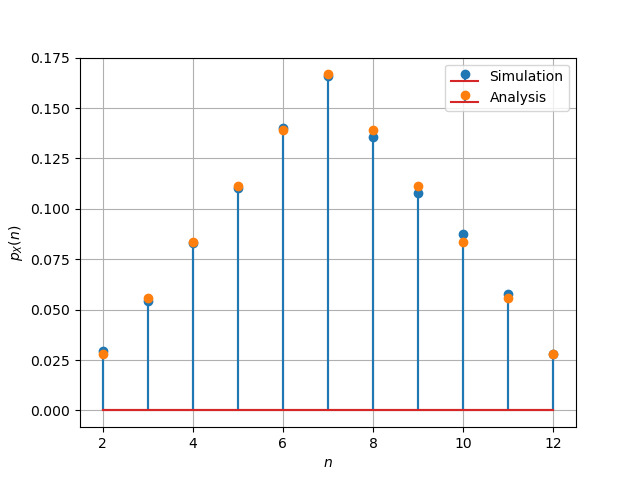
\includegraphics[scale = 0.5]{chapters/figs/pmf.png}
\caption{Plot of $p_X(n)$.  Simulations are close to the analysis. }
\label{fig:dice}
\end{figure}
\item The python code is available in 
\begin{lstlisting}
	chapters/codes/dice.py
\end{lstlisting}
\end{enumerate}


\newpage
\chapter{Random Numbers}
\section{Uniform Random Numbers}
Let $U$ be a uniform random variable between 0 and 1.
\begin{enumerate}
\item Generate $10^6$ samples of $U$ using a C program and save into a file called uni.dat .
\label{prob:uni_gen}
\\
\solution Download the following files and execute the  C program.
\begin{lstlisting}
	chapter2/codes/exrand.c
    chapter2/codes/coeffs.h
\end{lstlisting}

%
\item
Load the uni.dat file into python and plot the empirical CDF of $U$ using the samples in uni.dat. The CDF is defined as
\begin{align}
F_{U}(x) = \pr{U \le x}
\end{align}

\begin{lstlisting}
chapter2/codes/cdf_plot.py	
\end{lstlisting}
\begin{figure}[H]
\centering
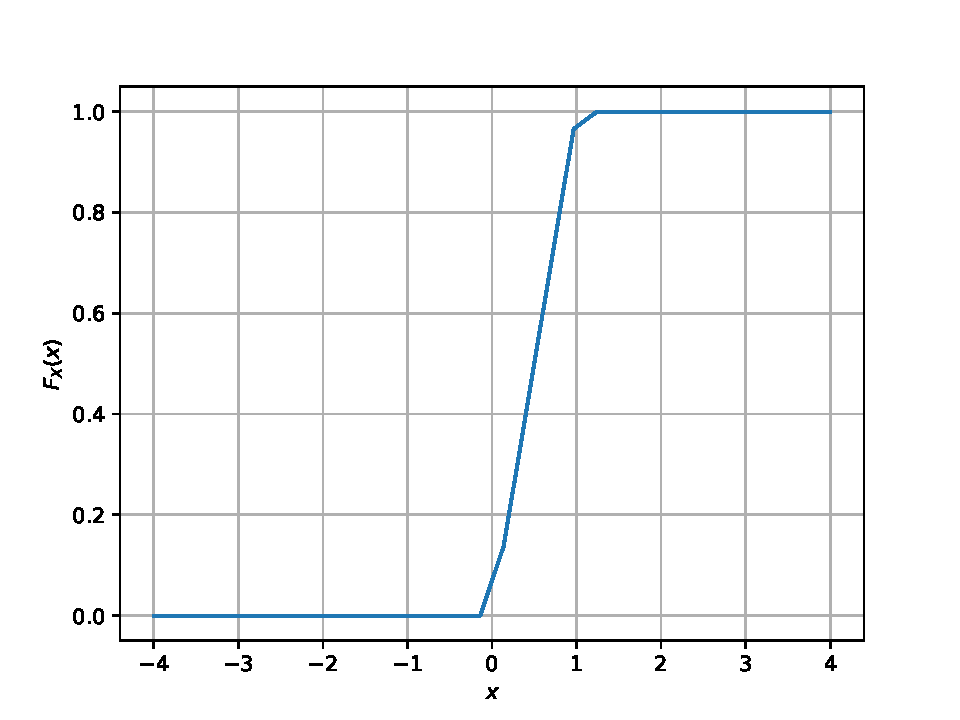
\includegraphics[scale=0.8]{chapter2/figs/uni_cdf.pdf}
\caption{The CDF of $U$}
\label{fig:uni_cdf}
\end{figure}
\item
Find a  theoretical expression for $F_{U}(x)$.\\
\solution
%\begin{align} 
%F_{U}(x) = \int_{-\infty}^{x} f_{U}(x)\,dx
%\label{eq:pdf_to_cdf}
%\end{align}
%For the uniform random variable $U$, $f_{U}(x)$ is given by  
%\begin{align}
%	f_U(x) &= 
%	\begin{cases}
%	1 &  0 \le x \le  1
%	\\
%	0 & elsewhere
%	\\
%	\end{cases}
%	\label{eq:uni_pdf}
%\end{align}
%Substituting \eqref{eq:uni_pdf} in \eqref{eq:pdf_to_cdf}, $F_U(x)$ is found to be
\begin{align}
	F_U(x) &= 
	\begin{cases}
	0 & x < 0
	\\	
	x & 0 \le x \le  1
	\\
	1 & x > 0
	\\
	\end{cases}
	\label{eq:uni_cdf}
\end{align}

\item
\label{prob:print_uni}
The mean of $U$ is defined as
%
\begin{equation}
E\sbrak{U} = \frac{1}{N}\sum_{i=1}^{N}U_i
\end{equation}
%
and its variance as
%
\begin{equation}
\text{var}\sbrak{U} = E\sbrak{U- E\sbrak{U}}^2 
\end{equation}

Write a C program to  find the mean and variance of $U$.\\
\solution The code below is the function for calculating mean
\begin{lstlisting}
	double mean(char *str)
{
int i=0,c;
FILE *fp;
double x, temp=0.0;

fp = fopen(str,"r");
//get numbers from file
while(fscanf(fp,"%lf",&x)!=EOF)
{
//Count numbers in file
i=i+1;
//Add all numbers in file
temp = temp+x*x;
}
fclose(fp);
temp = temp/(i-1);
return temp;

}
\end{lstlisting}
Function for calculating the mean
\begin{lstlisting}
double variance(char *str)
{
int i=0,c;
FILE *fp;
double x, sum_square=0.0, temp=0.0, var;

fp = fopen(str,"r");
//get numbers from file
while(fscanf(fp,"%lf",&x)!=EOF)
{
//Count numbers in file
i=i+1;
//Add all numbers in file
temp += x;
sum_square += (x*x);
}
fclose(fp);
var = (sum_square - temp*temp/(i-1))/(i-2);
return var;

}
\end{lstlisting}
The following code prints the mean and variance of $U$
\begin{lstlisting}
	chapter2/codes/mv.c
\end{lstlisting}
The output of the program is
\begin{lstlisting}
Uniform stats:
Mean: 0.500007
Variance: 0.083301
\end{lstlisting}

\item Verify your result theoretically given that
%
\begin{equation}
E\sbrak{U^k} = \int_{-\infty}^{\infty}x^kdF_{U}(x)
\end{equation}\\
\solution For a random variable $X$, the mean $\mu_X$ is given by
\begin{align}
	\label{eq:mean_exp}
	\mu_X &= E\sbrak{X} = \int_{-\infty}^{\infty}xdF_{U}(x) \\
	\label{eq:var_exp}
	\sigma_X^2 &= E\sbrak{X^2} - \mu_X^2 = \int_{-\infty}^{\infty}x^2dF_{U}(x) - \mu_X^2
\end{align} 
Variance $\sigma_X^2$ is given by
 
Substituting the CDF of $U$ from (2.1.3.3) in (2.1.5.2) and (2.1.5.3), we get \\
 \begin{align}
	\label{eq:mean_uni}
	\textbf{Mean} & =\mu_U & \\
 \mathrm{E}[X]=\int_a^b x \cdot \frac{1}{b-a} d x
 \\ Here \  a=0,b=1
 \\ \mu= \mathrm{E}[X]= \frac{1}{2} = 0.5	\\
	\label{eq:var_uni}
	\mathrm{E}[X^2]=\int_a^b x^2 \cdot \frac{1}{b-a} d x=\frac{b^3-a^3}{3} \cdot \frac{1}{b-a} \\
 \text{Variance} \\
 \sigma^2=E\left(X^2\right)-[E(X)]^2
 =\frac{(a-b)^2}{12}\\
  \sigma^2 = \frac{1}{12} & = 0.08
\end{align} 
Hence, the output values of program and theory are same.
\end{enumerate}
\section{Central Limit Theorem}
\begin{enumerate}
\item
Generate $10^6$ samples of the random variable
%
\begin{equation}
X = \sum_{i=1}^{12}U_i -6
\end{equation}
%
using a C program, where $U_i, i = 1,2,\dots, 12$ are  a set of independent uniform random variables between 0 and 1
and save in a file called gau.dat\\
\solution Use the following code and it will generate gau.dat file with the required Random variables the  C program.
\begin{lstlisting}
	chapter2/codes/rv.c
\end{lstlisting}
%
\item
Load gau.dat in python and plot the empirical CDF of $X$ using the samples in gau.dat. What properties does a CDF have?
\\
\begin{figure}[h!]
\centering
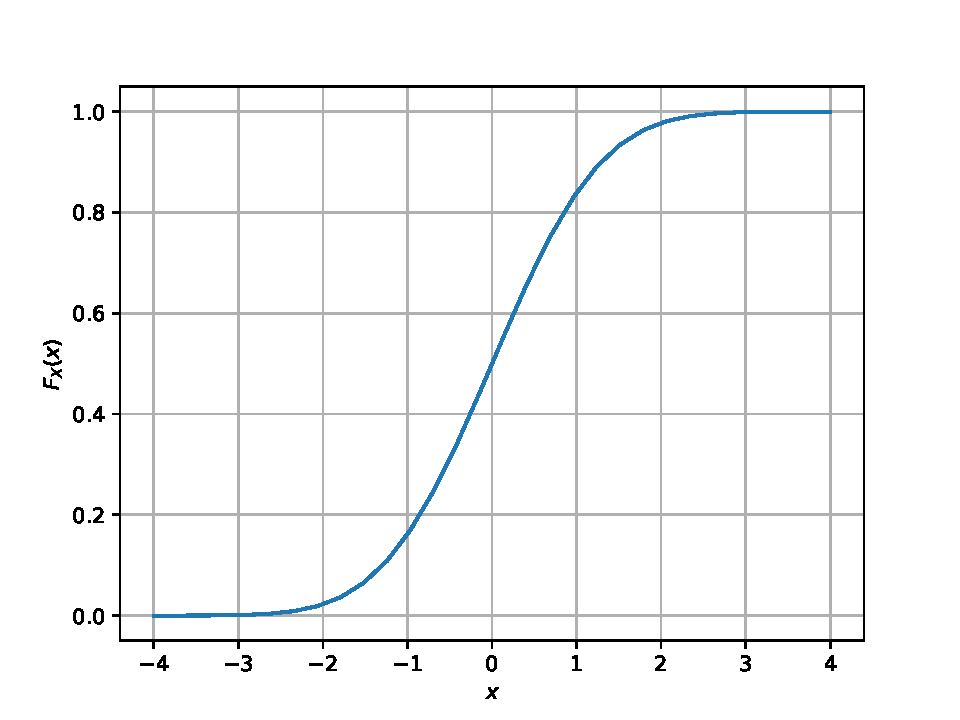
\includegraphics[scale=0.8]{chapter2/figs/gauss_cdf.pdf}
\caption{The CDF of $X$}
\label{fig:gauss_cdf}
\end{figure}
Let $X$ be a random variable (either continuous or discrete), then the CDF
of $X$ has the following properties \\
The CDF is a non-decreasing \\
The maximum of the CDF is when
\begin{eqnarray}
x = \infty: F_X(\infty) = 1
\end{eqnarray}
The minimum of the CDF is when
\begin{eqnarray}
x = -\infty: F_X(-\infty) = 0	
\end{eqnarray} 
If the CDF $F_X$ is continuous at any
$a \le x \le b$, then
\begin{eqnarray}
\Pr \lsbrak a \le X \le \rsbrak b  = F_X (b) - F_X (a)
\end{eqnarray}
For any random variable X (discrete or continuous), $P[X = b]$ is
\begin{eqnarray}
\Pr \lsbrak X = \rsbrak b = 
\begin{cases}
	F_X (b) - F_X (b-) & \text{if $F_X$ is discontinuous at x = b}
	\\	
	0 & otherwise
	\\
	\end{cases}
\end{eqnarray}
\item
Load gau.dat in python and plot the empirical PDF of $X$ using the samples in gau.dat. The PDF of $X$ is defined as
\begin{align}
p_{X}(x) = \frac{d}{dx}F_{X}(x)
\label{eq:cdf_to_pdf}
\end{align}
What properties does the PDF have?
\solution 
\begin{lstlisting}
	chapter2/codes/rv.c
\end{lstlisting}

\begin{figure}[h!]
\centering
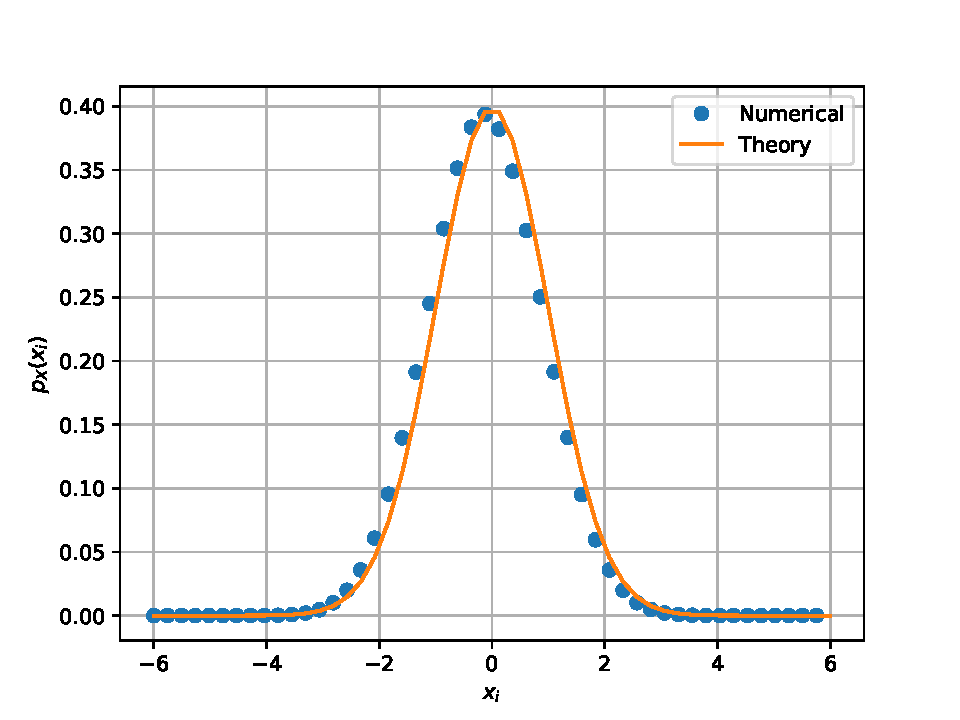
\includegraphics[scale=0.8]{chapter2/figs/gauss_pdf.pdf}
\caption{The PDF of $X$}
\label{fig:gauss_pdf}
\end{figure}

The properties of PDF are
\begin{eqnarray}
	f_X(x) \ge 0 \text{for all} X \in \mathbb{R} \\
	\int_{-\infty}^{\infty} f_X(x) \,dx = 1
\end{eqnarray}

\item Find the mean and variance of $X$ by writing a C program.  \\
\solution The following code prints the mean and variance of $X$
\begin{lstlisting}
	chapter2/codes/mean.c
\end{lstlisting}
The output of the program is
\begin{lstlisting}
Gaussian stats:
Mean: 0.000294
Variance: 0.999561	
\end{lstlisting}
\item Given that 
\begin{align}
p_{X}(x) = \frac{1}{\sqrt{2\pi}}\exp\brak{-\frac{x^2}{2}}, -\infty < x < \infty,
\label{eq:gau_pdf}
\end{align}
repeat the above exercise theoretically.\\
\solution The mean of gievn PDF is given by $E\sbrak{X}$ ,
\begin{flalign}
	E\sbrak{X} = \mu_X &= \int_{-\infty}^{\infty} \frac{1}{\sqrt{2\pi}}\exp\brak{-\frac{x^2}{2}} \,dx&\\
     = \frac{1}{\sqrt{2\pi}} \int_{-\infty}^{\infty} x e^{-\frac{x^2}{2}}dx\\
    &=0 & \\ 
	\mu_X &= 0
\end{flalign}
Variance is given by
\begin{align}
    \sigma^2 =  E\brak X^2 - E^2\brak X 
\end{align}
Substituting $\mu_X$ and the PDF
\begin{flalign}
	 &= \frac{1}{\sqrt{2\pi}} \int_{0}^{\infty} x^2 e^{-\frac{x^2}{2}} dx\\
    &= \frac{2}{\sqrt{2\pi}}\int_{0}^{\infty}\sqrt{2u}e^{-u} du \quad\brak{Let \frac{x^2}{2}= u}\\
    &= \frac{2}{\sqrt{\pi}} \int_{0}^{\infty} e^{-u} u^{\frac{3}{2}-1} du \quad\brak{Let \Gamma\brak{\frac{1}{2}}=\sqrt{\pi}}\\
    &= \frac{2}{\sqrt{\pi}} \Gamma\brak{{\frac{3}{2}}}\\
    &= \frac{1}{\sqrt{\pi}}\Gamma\brak{\frac{1}{2}} \\
    &= 1
\end{flalign}
%
\end{enumerate}


\section{From Uniform to Other}
\begin{enumerate}
%
\item
Generate samples of 
%
\begin{equation}
V = -2\ln\brak{1-U}
\end{equation}
%
and plot its CDF. \\
\solution
\begin{lstlisting}
	chapter2/2_3_cdf.py
\end{lstlisting}
\begin{figure}[H]
\centering
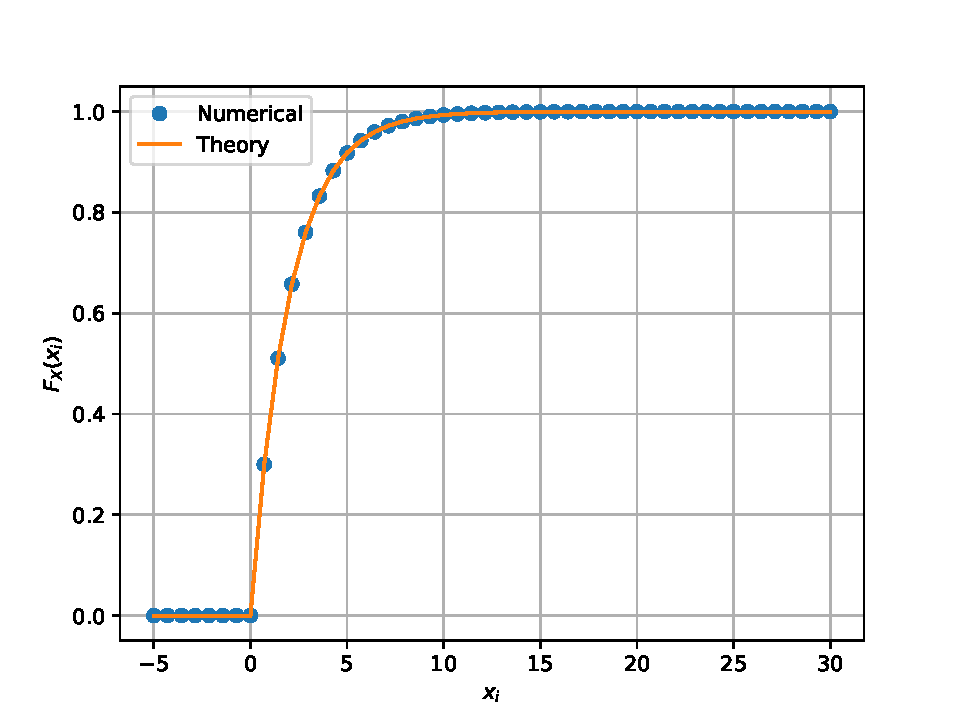
\includegraphics[scale = 0.7]{chapter2/figs/log.pdf}
\caption{The CDF of $V$}
\label{fig:log_uni_cdf}
\end{figure}
\item Find a theoretical expression for $F_V(x)$.
\begin{flalign}
	F_V(x) &= P(V \le x)&\\
	&= P(-2\ln\brak{1-U} \le x)&\\
	&= P(U \le 1 - e^{\frac{-x}{2}})&\\
	&= F_U(1 - e^{\frac{-x}{2}})
	\label{eq:probman_cdf_V_temp}
\end{flalign}
\begin{align}
F_U(x) = 
\begin{cases}
0 &  x < 0 \\
x & 0 \le x \le 1 \\
1 & x > 1
\end{cases}
\end{align}
%
Substituting the above in \eqref{eq:probman_cdf_V_temp},
%
\begin{align}
F_U\brak{1- e^{-\frac{x}{2}}} =
\begin{cases}
0 &  1- e^{-\frac{x}{2}} < 0 \\
1- e^{-\frac{x}{2}} & 0 \le 1- e^{-\frac{x}{2}} \le 1 \\
1 & 1- e^{-\frac{x}{2}} > 1
\end{cases}
\end{align}
After some algebra, the above conditions yield
\begin{align}
F_V(x) = 
\begin{cases}
0 & x < 0 \\
1- e^{-\frac{x}{2}} & x \ge 0
\end{cases}
\label{eq:probman_V_cdf_anal}
\end{align}
\end{enumerate}


\section{Triangular Distribution}
%
\begin{enumerate}
\item Generate 
	\begin{align}
		T = U_1+U_2
	\end{align}\\
\solution Download the following files and execute the  C program.
\begin{lstlisting}
chapter2/codes/tri.c
\end{lstlisting}
\item Find the CDF of $T$.\\
\solution 
\begin{lstlisting}
	chapter2/codes/tcdf.py
\end{lstlisting}
\begin{figure}[H]
\centering
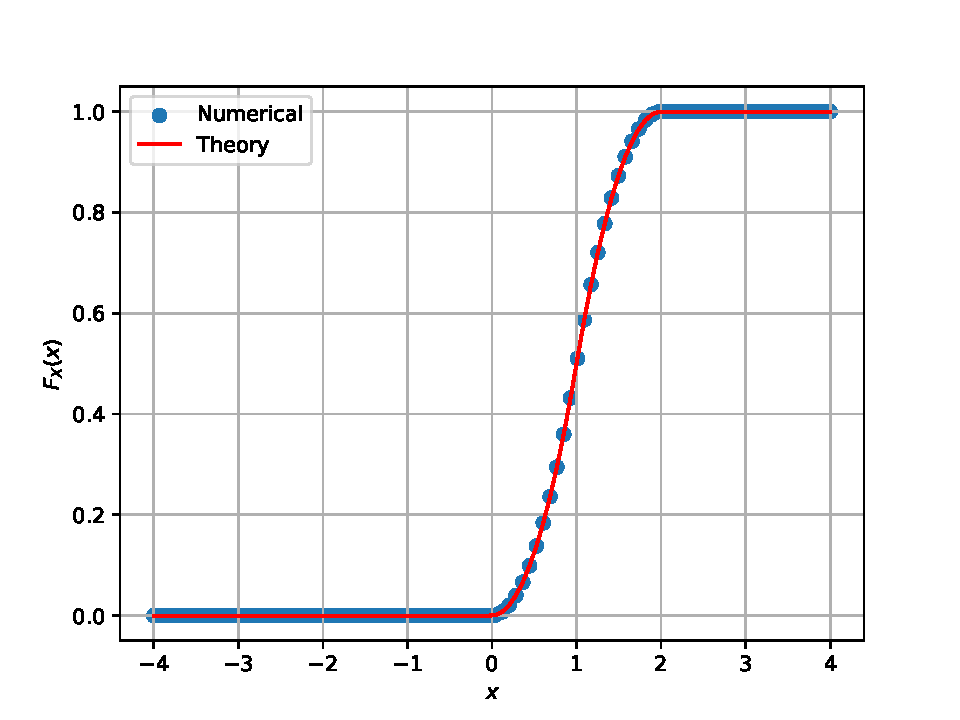
\includegraphics[scale=0.8]{chapter2/figs/triangle_cdf.pdf}
\caption{The CDF of $T$}
\label{fig:tri_cdf}
\end{figure}
\item Find the PDF of $T$.\\

\begin{lstlisting}
chapter2/codes/tdpf.py
\end{lstlisting}
\begin{figure}[H]
\centering
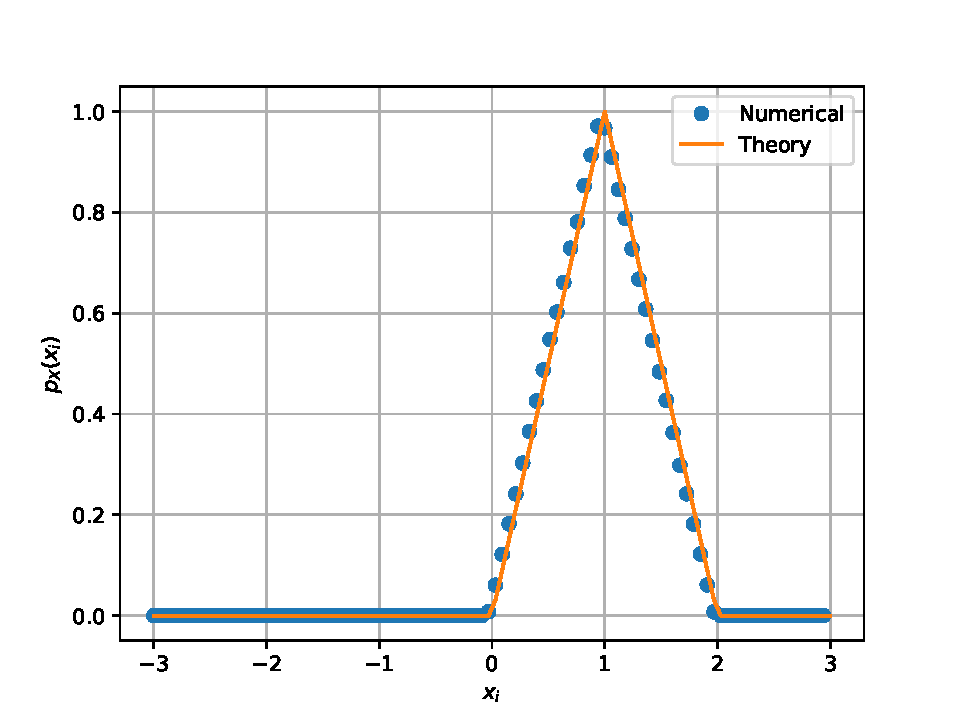
\includegraphics[scale=0.8]{chapter2/figs/triangle_pdf.pdf}
\caption{The PDF of $T$}
\label{fig:tri_pdf}
\end{figure}
\item Find the theoretical expressions for the PDF and CDF of $T$.\\
\solution 

CDF $F_U(x)$ is
\begin{align}
F_{T}(x) &= 
\begin{cases}
0 & x \leq a \\
\frac{(x-a)^2}{(b-a)(c-a)} & a < x \leq c \\
1-\frac{(b-x)^2}{(b-a)(c-a)} & c < x \leq b\\
1 & x > b
\end{cases}
\end{align}
PDF $p_T(x)$
\begin{align}
p_{T}(x) = \frac{d}{dx}F_{T}(x)
\end{align}
\begin{align}
p_{T}(x) &= 
\begin{cases}
0 & x \leq a \\
\frac{2(x-a)}{(b-a)(c-a)} & a < x \leq c \\
\frac{2(b-x)}{(b-a)(c-a)} & c < x \leq b\\
0 & x > b
\end{cases}
\end{align}

\item Verify your results through a plot. \\
\solution Refer the \figref{fig:tri_cdf} and \figref{fig:tri_pdf}
\end{enumerate}

\newpage
\chapter{Maximum Likelihood Detection: BPSK}

\section{Maximum Likelihood}
\begin{enumerate}
\item Generate equiprobable $X \in \cbrak{1,-1}$.\\
\solution $X$ can be generated in python using the below code section,
\begin{lstlisting}
	chapter3/codes/eqi_prob.py
\end{lstlisting}
\item Generate 
\begin{equation}
Y = AX+N,
\end{equation}
where $A = 5$ dB,  and $N \sim \gauss{0}{1}$.\\
\solution $Y$ can be generated in python using the below code section,
\begin{lstlisting}
	chapter3/codes/Y_gau.py
\end{lstlisting}
\item Plot $Y$ using a scatter plot.\\
\solution 
\begin{lstlisting}
		chapter3/codes/scatter.py
\end{lstlisting}
\begin{figure}[H]
\centering
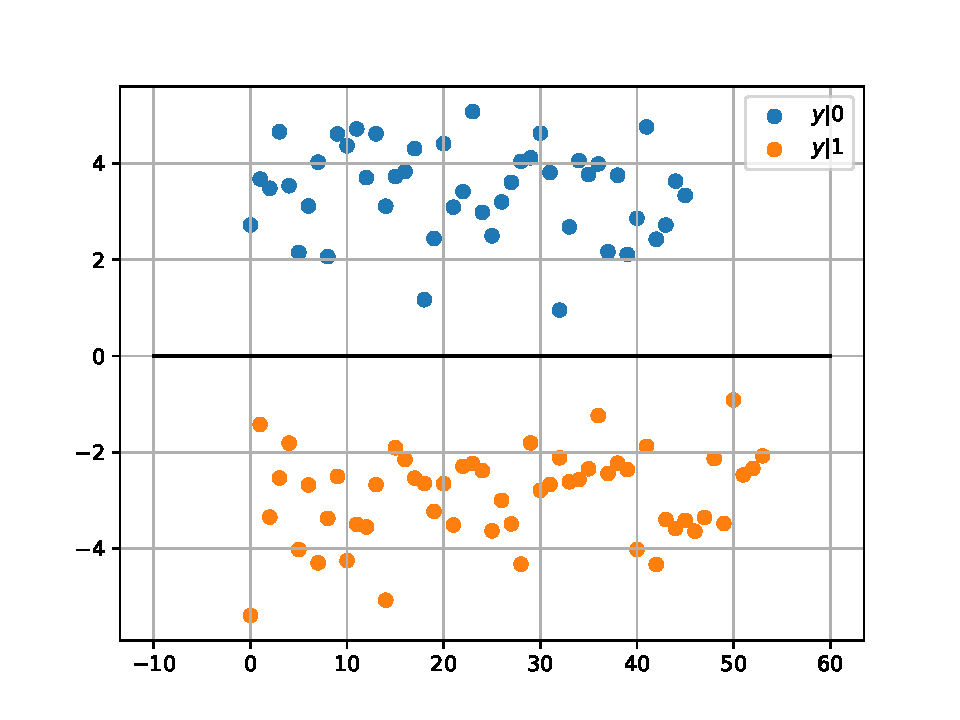
\includegraphics[width=\columnwidth]{chapter3/figs/bpsk_scatter.pdf}
\caption{Scatter plot of $Y$}
\label{fig:bpsk_scatter}
\end{figure}
\item Guess how to estimate $X$ from $Y$.\\
\solution
\begin{equation}
y \dec{1}{-1} 0
\label{eq:bpsk_decision}
\end{equation}
\item
\label{ml-ch4_sim}
Find 
\begin{equation}
	P_{e|0} = \pr{\hat{X} = -1|X=1}
\end{equation}
and 
\begin{equation}
	P_{e|1} = \pr{\hat{X} = 1|X=-1}
\end{equation}\\
\solution
\begin{flalign*}
	\pr{\hat{X} = -1|X=1} &= \pr{Y < 0|X=1}&\\
	&= \pr{AX + N < 0|X=1}&\\ 
	&= \pr{A + N < 0}&\\
	&= \pr{N < -A}
\end{flalign*}
Similarly,
\begin{flalign*}
	\pr{\hat{X} = 1|X=-1} &= \pr{Y > 0|X=-1}&\\
	&= \pr{N > A}
\end{flalign*}
Since $N \sim \gauss{0}{1}$,
\begin{flalign}
	\label{eq:std_norm_symmetric}
	\pr{N < -A} &= \pr{N > A}&\\
	\label{eq:bpks_prob_err_cond}
	\implies P_{e|0} &= P_{e|1} = \pr{N > A}
\end{flalign}
%
\item Find $P_e$ assuming that $X$ has equiprobable symbols.\\
\solution
\begin{flalign}
	P_e &= \pr{X=1}P_{e|1} + \pr{X=-1}P_{e|0}&\\
	\intertext{Since $X$ is equiprobable}\\
	\label{eq:bpsk_prob_error_equi}
	P_e &= \frac{1}{2}P_{e|1} + \frac{1}{2}P_{e|0}
\end{flalign}
Substituting from \eqref{eq:bpks_prob_err_cond}
\begin{equation}
	P_e = \pr{N > A}
\end{equation}
Given a random varible $X \sim \gauss{0}{1}$ the Q-function is defined as
\begin{align}
	Q(x) &= \pr{X > x}\\
	\label{eq:q_func_integral}
	Q(x) &= \frac{1}{\sqrt{2\pi}} \int_x^\infty \exp\left(-\frac{u^2}{2}\right) \, du.\\
\end{align}
Using the Q-function, $P_e$ is rewritten as
\begin{equation}
	P_e = Q(A)
\end{equation} 
%
\item
Verify by plotting  the theoretical $P_e$ with respect to $A$ from 0 to 10 dB.\\
\solution 
\begin{lstlisting}
		chapter3/codes/bpsk_pe.py
\end{lstlisting}
\begin{figure}[H]
\centering
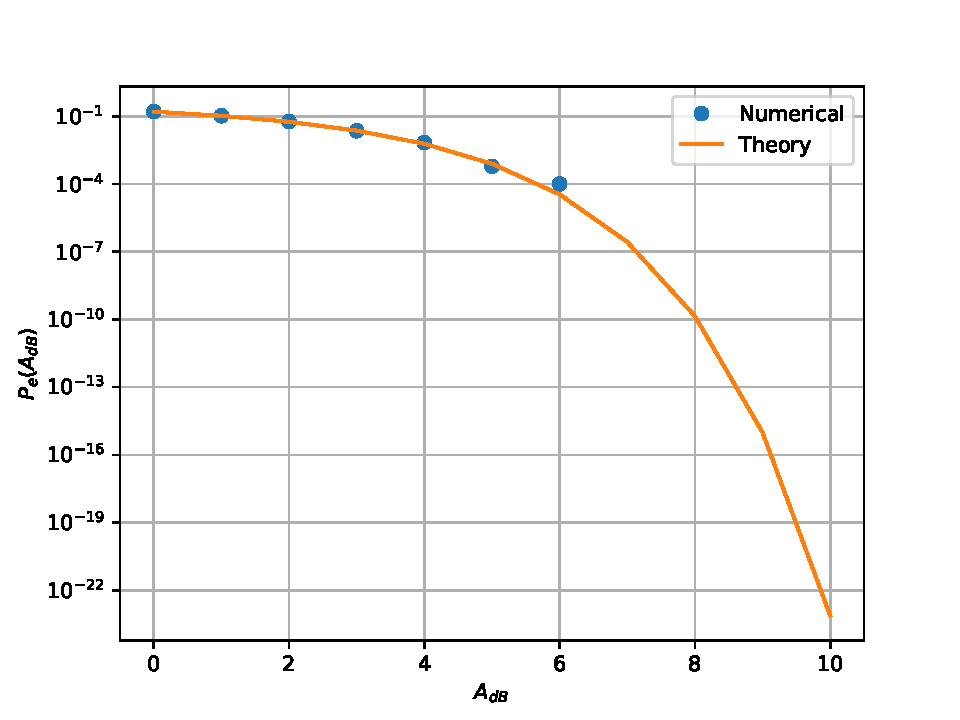
\includegraphics[width=\columnwidth]{chapter3/figs/bpsk_pe_snr.pdf}
\caption{$P_e$ versus $A$ plot}
\label{fig:bpsk_pe_snr}
\end{figure}
%
\item Now, consider a threshold $\delta$  while estimating $X$ from $Y$. Find the value of $\delta$ that maximizes the theoretical $P_e$.\\
\label{prob:bpsk_delta_equi}
\solution Given the decision rule, 
\begin{equation}
y \dec{1}{-1} \delta
\label{eq:bpsk_decision_delta}
\end{equation}
\begin{flalign*}
	P_{e|0} &= \pr{\hat{X} = -1|X=1}&\\
	&= \pr{Y < \delta|X=1}&\\
	&= \pr{AX + N < \delta|X=1}&\\ 
	&= \pr{A + N < \delta}&\\
	&= \pr{N < -A + \delta}&\\
	&= \pr{N > A - \delta}&\\
	&= Q(A-\delta)
\end{flalign*}
\begin{flalign*}
	P_{e|1} &= \pr{\hat{X} = 1|X=-1}&\\
	&= \pr{Y > \delta|X=-1}&\\
	&= \pr{N > A + \delta}&\\
	&= Q(A+\delta)
\end{flalign*}
Using \eqref{eq:bpsk_prob_error_equi}, $P_e$ is given by
\begin{flalign}
	P_e &= \frac{1}{2}Q(A+\delta) + \frac{1}{2}Q(A-\delta)
\end{flalign}
Using the integral for Q-function from \eqref{eq:q_func_integral},
\begin{align}
	\label{eq:prob_error_delta_equi}
	P_e &= k(\int_{A+\delta}^\infty \exp\left(-\frac{u^2}{2}\right) \, du + \int_{A-\delta}^\infty \exp\left(-\frac{u^2}{2}\right) \, du)\\
	\intertext{where k is a constant}	\nonumber
\end{align}
Differentiating \eqref{eq:prob_error_delta_equi} wrt $\delta$ (using Leibniz's rule) and equating to $0$, we get
\begin{flalign*}
	\exp\left(-\frac{(A+\delta)^2}{2}\right)-\exp\left(-\frac{(A-\delta)^2}{2}\right) &= 0&\\
	\frac{\exp\left(-\frac{(A+\delta)^2}{2}\right)}{\exp\left(-\frac{(A\delta)^2}{2}\right)} &= 1&\\
	\exp\left(-\frac{(A+\delta)^2-(A-\delta)^2}{2}\right) &= 1&\\
	\exp\left(-2A\delta\right) &= 1&\\
	\intertext{Taking $\ln$ on both sides}\\
	-2A\delta &= 0&\\
	\implies \delta &= 0
\end{flalign*}
$P_e$ is maximum for $\delta = 0$
\item Repeat the above exercise when 
\label{prob:bpsk_decision_uneqi}
	\begin{align}
		p_{X}(0) = p
	\end{align}\\
\solution Since $X$ is not equiprobable, $P_e$ is given by,
\begin{flalign}
	P_e &= (1-p)P_{e|1} + pP_{e|0}&\\
	&= (1-p)Q(A+\delta) + pQ(A-\delta)
\end{flalign}
Using the integral for Q-function from \eqref{eq:q_func_integral},
\begin{multline}
	\label{eq:prob_error_delta_nonequi}
	P_e = k((1-p)\int_{A+\delta}^\infty \exp\left(-\frac{u^2}{2}\right) \, du + \\
	p\int_{A-\delta}^\infty \exp\left(-\frac{u^2}{2}\right) \, du)
\end{multline}
where $k$ is a constant.\\
Following the same steps as in problem \ref{prob:bpsk_delta_equi}, $\delta$ for maximum $P_e$ evaluates to,
\begin{equation}
	\delta = \frac{1}{2A}\ln\left(\frac{1}{p}-1\right)
\end{equation}
\item Repeat the above exercise using the MAP criterion.\\
\solution 
The MAP rule can be stated as\\
\begin{flalign}
\label{eq:map_rule}
\text{Set } \hat{x} &= x_i \text{ if}&\\ \nonumber
p_X(x_k)p_Y(y|x_k) &\text{ is maximum for } k = i
\end{flalign}
For the case of BPSK, the point of equality between $p_X(x=1)p_Y(y|x=1)$ and $p_X(x=-1)p_Y(y|x=-1)$ is the optimum threshold. If this threshold is $\delta$, then
\begin{flalign*}
	pp_Y(y|x=1) > (1-p)p_Y(y|x=-1) &\text{ when } y > \delta&\\
	pp_Y(y|x=1) < (1-p)p_Y(y|x=-1) &\text{ when } y < \delta 	
\end{flalign*}
The above inequalities can be visualized in \figref{fig:bpsk_map_density} for $p = 0.3$ and $A = 3$.
\begin{figure}[H]
\centering
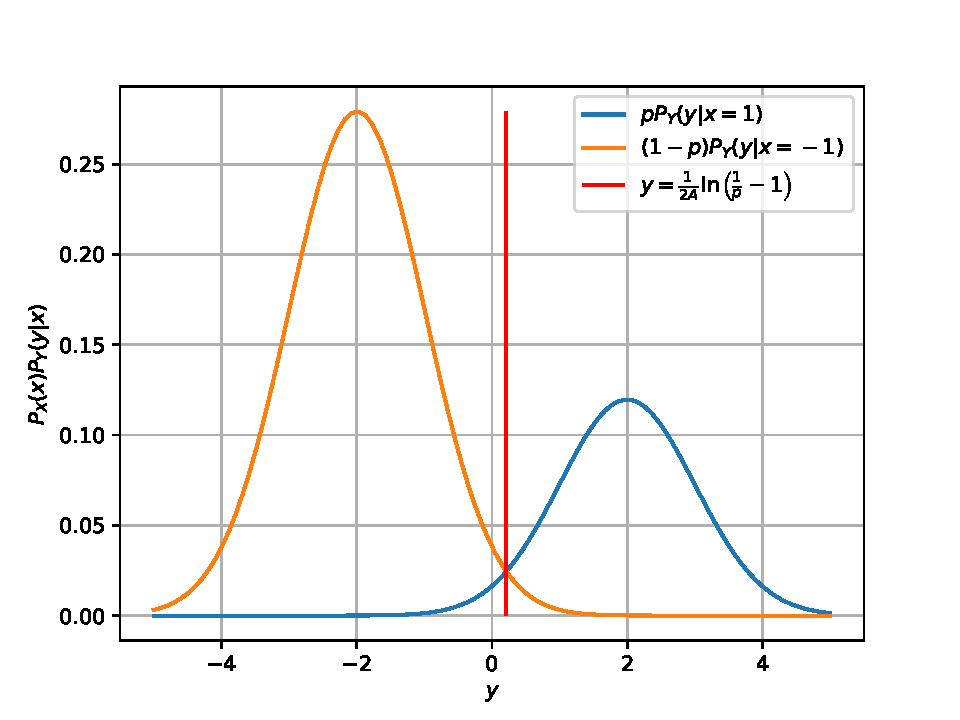
\includegraphics[width=\columnwidth]{chapter3/figs/bpsk_map_density.pdf}
\caption{$p_X(X=x_i)p_Y(y|x=x_i)$ versus $y$ plot for $X \in \{-1,1\}$}
\label{fig:bpsk_map_density}
\end{figure}
Given $Y=AX+N$ where $N \sim \gauss{0}{1}$, the optimum threshold is found as solution to the below equation
\begin{equation}
	p\exp\left(-\frac{(y_{eq}-A)^2}{2}\right) = (1-p)\exp\left(-\frac{(y_{eq}+A)^2}{2}\right)
\end{equation}
Solving for $y_{eq}$, we get
\begin{equation}S
	y_{eq} = \delta = \frac{1}{2A}\ln\left(\frac{1}{p}-1\right)
\end{equation}
which is same as $\delta$ obtained in problem \ref{prob:bpsk_decision_uneqi}

\begin{lstlisting}
		chapter3/codes/map.py	
\end{lstlisting}
\end{enumerate}-

\newpage
\chapter{Transformation of Random Variables}
\section{Gaussian to Other}
\begin{enumerate}
\item
Let $X_1 \sim  \gauss{0}{1}$ and $X_2 \sim  \gauss{0}{1}$. Plot the CDF and PDF of
%
\begin{equation}
V = X_1^2 + X_2^2
\end{equation}\\
\solution Refer The CDF and PDF of $V$ plots in \figref{fig:chisq_cdf} and \figref{fig:chisq_pdf} 
\begin{lstlisting}
	chapter4/codes/sos.py
	chapter4/codes/sos1.py
\end{lstlisting}
\begin{figure}[H]
\centering
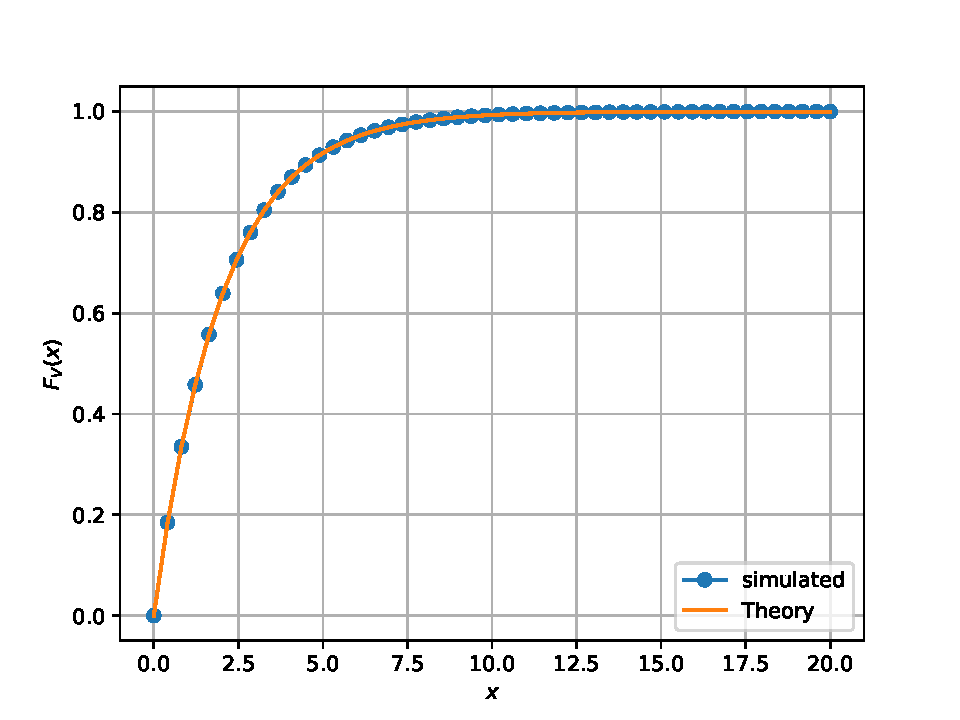
\includegraphics[scale=0.8]{chapter4/figs/chisq_cdf.pdf}
\caption{CDF of $V$}
\label{fig:chisq_cdf}
\end{figure}
\begin{figure}[H]
\centering
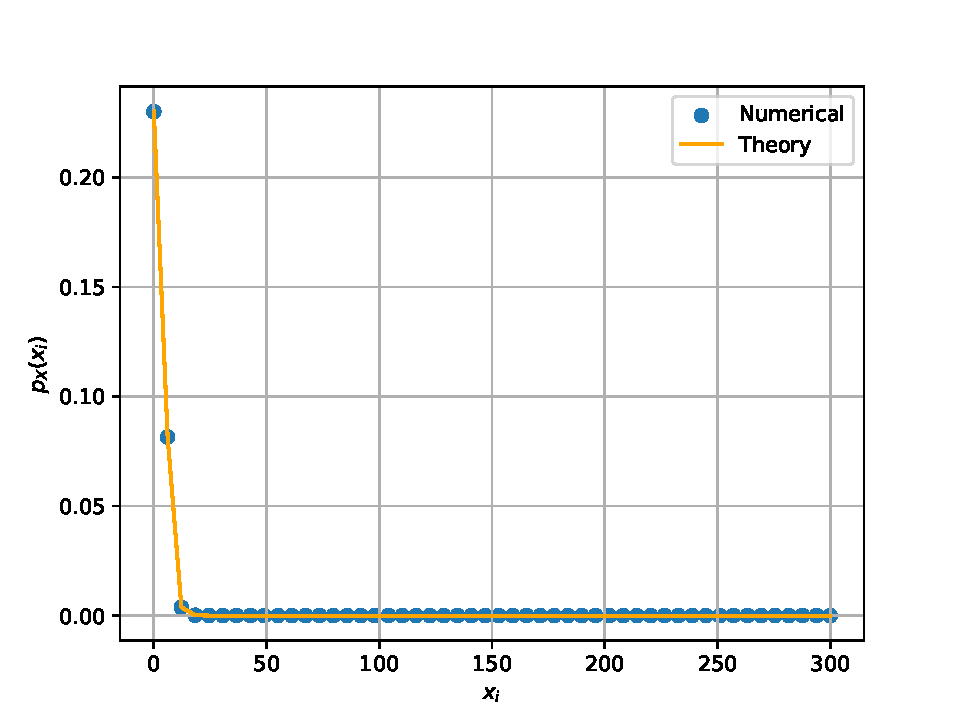
\includegraphics[scale=0.8]{chapter4/figs/chisq_pdf.pdf}
\caption{PDF of $V$}
\label{fig:chisq_pdf}
\end{figure}
%

%
%
\item
If
%
\begin{equation}
F_{V}(x) = 
\begin{cases}
1 - e^{-\alpha x} & x \geq 0 \\
0 & x < 0,
\end{cases}
\label{eq:chisq2_cdf_gen}
\end{equation}
%
find $\alpha$.\\
\solution 
%
\begin{lstlisting}
	chapter4/codes/cdf6.py
\end{lstlisting}
\begin{figure}
\centering
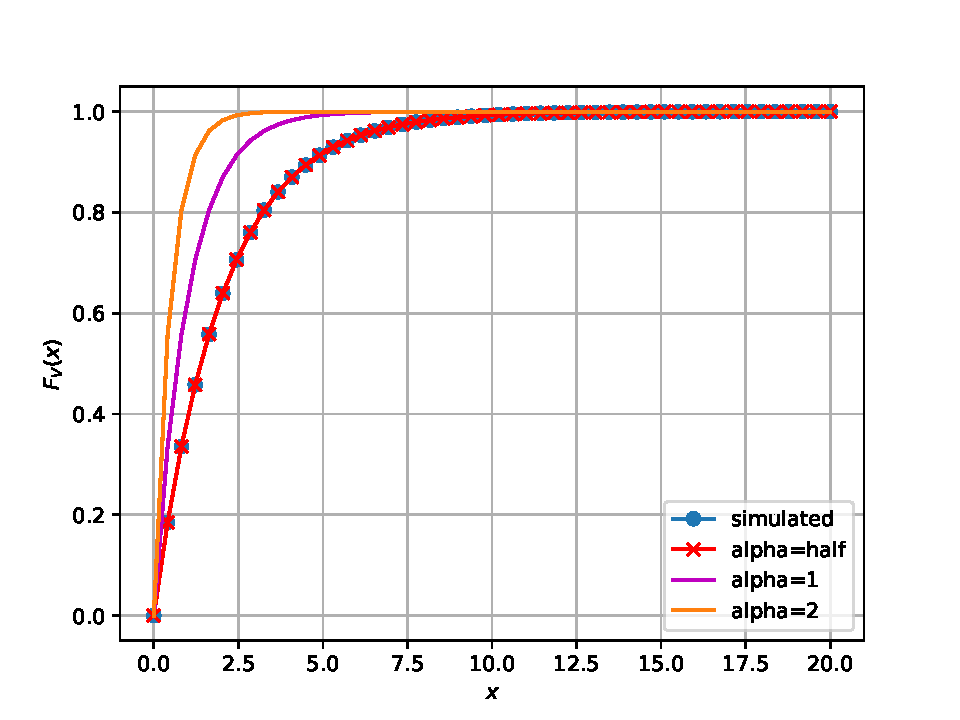
\includegraphics[scale=0.8]{chapter4/figs/cdf6.pdf}
\caption{The CDF of $V$ for different alpha}
\label{fig:gauss_cdf_alpha}
\end{figure}
from \ref{fig:gauss_cdf_alpha}
$alpha$= 0.5
\item
\label{ch3_raleigh_sim}
Plot the CDF and PDF of
%
\begin{equation}
A = \sqrt{V}
\end{equation}\\
\solution 
The CDF of $A$ is given by,
\begin{align}
	F_{A}\brak{a} &= \pr{A < a}\\
	&= \pr{\sqrt{V} < a}\\
	&= \pr{V < a^2}\\
	&= F_{V}\brak{a^2}\\
	&= 1-\exp\brak{-\frac{a^2}{2}} 
\end{align}
Using \eqref{eq:cdf_to_pdf}, the PDF is found to be
\begin{align}
	p_{A}\brak{a} &= a\exp\brak{-\frac{a^2}{2}}
\end{align}
\begin{lstlisting}
	chapter4/codes/cpdf.py
	chapter4/codes/cpdf1.py
\end{lstlisting}
\begin{figure}[H]
\centering
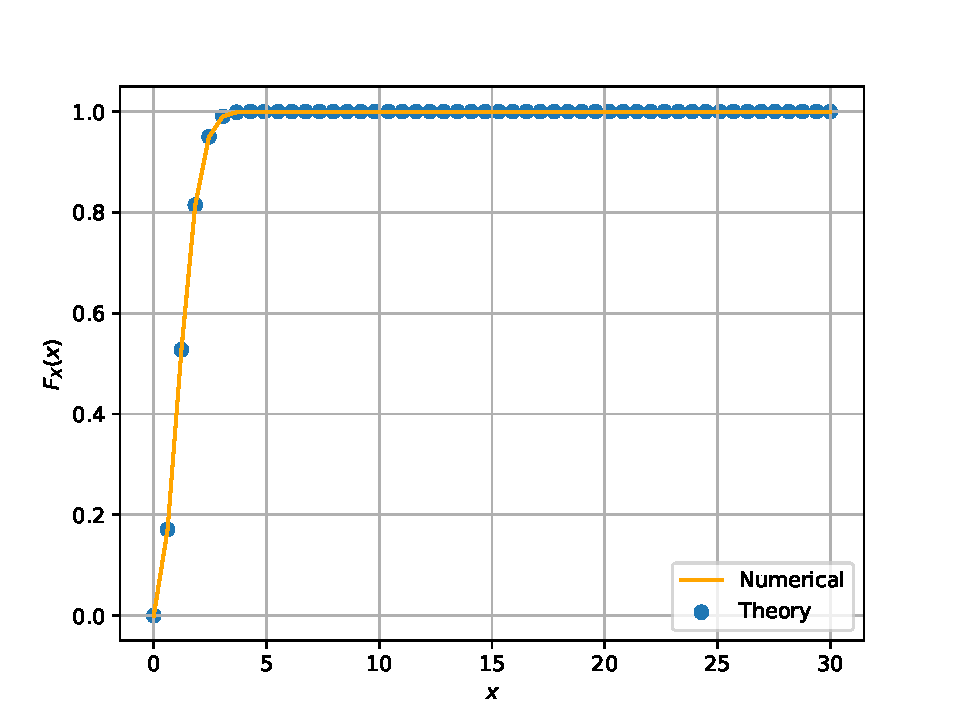
\includegraphics[scale = 0.8]{chapter4/figs/rayleigh_cdf.pdf}
\caption{CDF of $A$}
\label{fig:rayleigh_cdf}
\end{figure}
\begin{figure}[H]
\centering
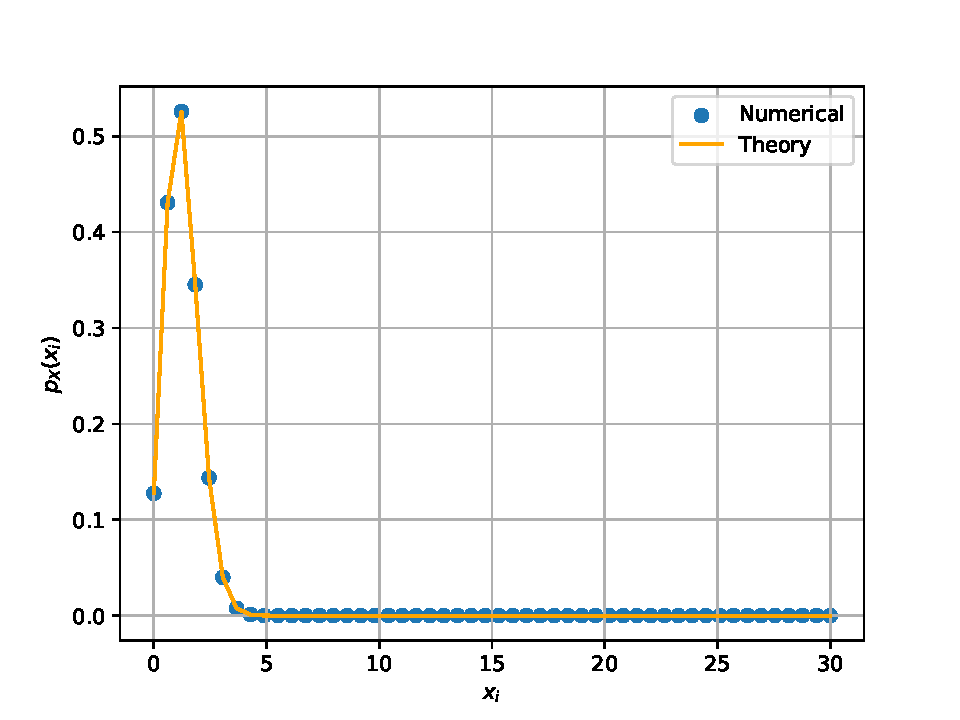
\includegraphics[scale=0.8]{chapter4/figs/rayleigh_pdf.pdf}
\caption{PDF of $A$}
\label{fig:rayleigh_pdf}
\end{figure}
%
\end{enumerate}

\section{Conditional Probability}
\begin{enumerate}
\item
\label{ch4_sim}
Plot 
\begin{equation}
P_e = \pr{\hat{X} = -1|X=1}
\end{equation}
%
for 
\begin{equation}
Y = AX+N,
\end{equation}
where $A$ is Raleigh with $E\sbrak{A^2} = \gamma, N \sim \gauss{0}{1}, X \in \brak{-1,1}$ for $0 \le \gamma \le 10$ dB.\\
\solution Refer \figref{fig:bpsk_pe_snr_rayleigh} 
\begin{lstlisting}
	chapter4/codes/cp.py
\end{lstlisting}
%
\item
Assuming that $N$ is a constant, find an expression for $P_e$.  Call this $P_e(N)$\\
\solution \solution The estimated value $\hat{X}$ is given by
\begin{align}
\hat{X} = 
\begin{cases}
+1 & Y>0\\
-1 & Y<0
\end{cases}
\end{align}
For $X = 1$, 
\begin{align}
Y &= A + N\\
P_e &= \pr{\hat{X} = -1|X=1} \\
&= \pr{Y<0 |X=1}\\
&= \pr{A<-N}\\
&= F_A(-N)\\
&= \int_{-\infty}^{-N} f_A(x)dx
\end{align}
By definition
\begin{align}
f_A(x) = 
\begin{cases}
\frac{x}{\sigma^2}\exp\brak{{-\frac{x^2}{2\sigma^2}}} & x\geq0\\
0 & otherwise
\end{cases}
\end{align}
If $N>0, f_A(x) = 0$. Then,
\begin{align}
 P_e=0  
\end{align}
If $N<0$. Then,
\begin{align}
 P_e(N) &=\int_{-\infty}^{-N} f_A(x)dx\\
 &=\int_{-\infty}^{0} 0dx+\int_{0}^{-N} f_A(x)dx\\
 &=\int_{0}^{-N} \frac{x}{\sigma^2}\exp\brak{{-\frac{x^2}{2\sigma^2}}}dx\\
 &=1-\exp{\brak{-\frac{N^2}{2\sigma^2}}}
\end{align}
Therefore,
\begin{align}\label{pe(N)}
P_e(N) = 
\begin{cases}
1-\exp\brak{{-\frac{N^2}{2\sigma^2}}} & N<0\\
0 & otherwise
\end{cases}
\end{align}
%
\item
%
\label{ch4_anal}
For a function $g$,
\begin{equation}
E\sbrak{g(X)} = \int_{-\infty}^{\infty}g(x)p_{X}(x)\, dx
\end{equation}
%
Find $P_e = E\sbrak{P_e(N)}$.\\
\solution Since $N \sim \gauss{0}{1}$ ,
\begin{align}
  p_N(x)= \frac{1}{\sqrt{2\pi}}\exp \brak{-\frac{x^2}{2} }
\end{align}
And from \eqref{pe(N)} 
\begin{align}
    P_e(x)=
    \begin{cases}
1-\exp\brak{{-\frac{x^2}{2\sigma^2}}} & x<0\\
0 & otherwise
\end{cases}
\end{align}

\begin{align}
 P_e=E\sbrak{P_e(N)} = \int_{-\infty}^{\infty}P_e(x)p_{N}(x)\, dx  
\end{align}
If $x<0, P_e(x)=0$ and using the fact that for an even function
\begin{align}
\int_{-\infty}^{\infty}f(x)=2\int_{-\infty}^{0}f(x)   
\end{align}
we get
\begin{align}
  P_e&= \frac{1}{\sqrt{2\pi}}\int_{-\infty}^{0}\exp \brak{ -\frac{x^2}{2}} \brak{1-\exp \brak{ -\frac{x^2}{2\sigma^2}} } dx\\
&= \frac{1}{2\sqrt{2\pi}} \int_{-\infty}^{\infty} \exp \brak{ -\frac{x^2}{2} }dx \nonumber \\
&- \frac{1}{2\sqrt{2\pi}} \int_{-\infty}^{\infty} \exp \brak{-\frac{(1+ \sigma^2)x^2}{2 \sigma^2}}  dx\\
&= \frac{\sqrt{2\pi} - \sqrt{\frac{\pi(2\sigma^2)}{1+\sigma^2}}}{2\sqrt{2\pi}}\\
&= \frac{1}{2} - \frac{1}{2}\sqrt{\frac{\sigma^2}{1+\sigma^2}}
\end{align}
For a Rayleigh Distribution with scale $= \sigma$,
\begin{align}
E\sbrak{A^2} = 2\sigma^2\\
\gamma = 2\sigma^2\\
\therefore P_e = \frac{1}{2} - \frac{1}{2}\sqrt{\frac{\gamma}{2+\gamma}}
\end{align}
%
\item
Plot $P_e$ in problems \ref{ch4_sim} and \ref{ch4_anal} on the same graph w.r.t $\gamma$.  Comment.\\
\solution $P_e$ plotted in same graph in \figref{fig:bpsk_pe_snr_rayleigh}. The value of $P_e$ is much higher when the channel %
gain $A$ is Rayleigh distributed than the case where $A$ is a constant (compare with \figref{fig:bpsk_pe_snr}).
\begin{figure}[H]
\centering
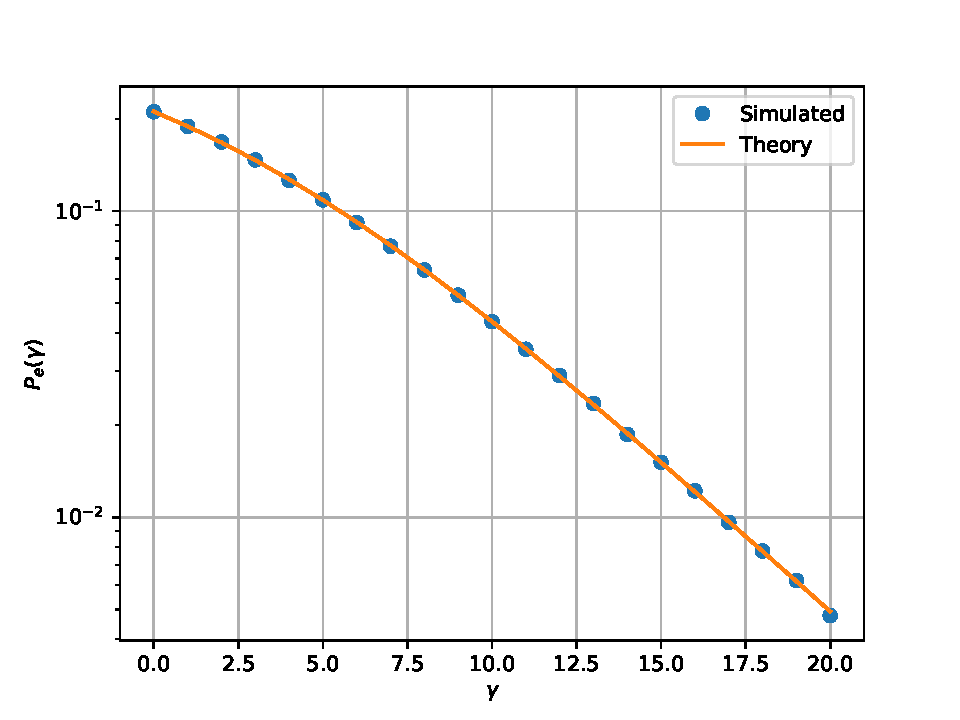
\includegraphics[scale=0.8]{chapter4/figs/prob_error.pdf}
\caption{$P_e$ versus $\gamma$}
\label{fig:bpsk_pe_snr_rayleigh}
\end{figure}
\end{enumerate}

\newpage
\chapter{Bivariate Random Variables: FSK}
\section{Two Dimensions}
Let 
\begin{equation}
\mbf{y} = A\mbf{x} + \mbf{n},
\end{equation}
where 
\begin{align}
x &\in \brak{\mbf{s}_0,\mbf{s}_1}, 
\mbf{s}_0 = 
\begin{pmatrix}
1 
\\
0
\end{pmatrix},
\mbf{s}_1 = 
\begin{pmatrix}
0 
\\
1
\end{pmatrix}
\\
\mbf{n} &= 
\begin{pmatrix}
n_1
\\
n_2
\end{pmatrix},
n_1,n_2 \sim \gauss{0}{1}.
\end{align}
%
\begin{enumerate}
%%
\item
\label{ch5_fsk}
Plot 
%
\begin{equation}
\mbf{y}|\mbf{s}_0 \text{ and } \mbf{y}|\mbf{s}_1
\end{equation}
%
on the same graph using a scatter plot.\\
\solution Refer \figref{fig:biv_scatter} for plot,
\begin{lstlisting}
chapter5/codes/biv_scatter.py
\end{lstlisting}
%
\begin{figure}[H]
\centering
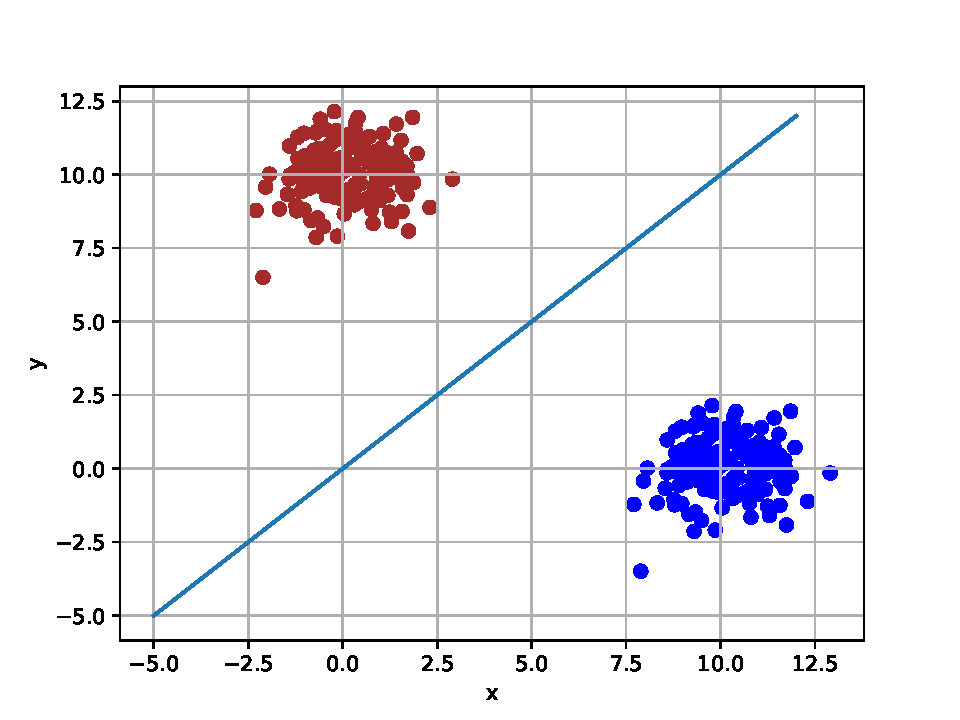
\includegraphics[scale=0.8]{chapter5/figs/biv_scatter.pdf}
\caption{Scatter plot of $\mbf{y}|\mbf{s}_0$ and $\mbf{y}|\mbf{s}_1$ }
\label{fig:biv_scatter}
\end{figure}

%
\item
For the above problem, find a decision rule for detecting the symbols $\mbf{s}_0 $ and $\mbf{s}_1$.\\
%\solution The multivariate Gaussian distribution is defined as
%
%\begin{multline}
%\label{eq:multivariate}
%p_{\mathbf{y}}(y_1,\dots,y_k)
%\\
%=\frac{1}{\sqrt{\brak{2\pi}^k\abs{\bm{\sigma}}}}\exp\cbrak{-\frac{1}{2}\brak{\mathbf{y}-\bm{\mu}}^T\bm{\sigma}^{-1}\brak{\mathbf{y}-\bm{\mu}}}
%\end{multline}
%%
%where $\bm{\mu}$ is the mean vector, $\bm{\sigma} = E\sbrak{\brak{\mathbf{x}-\bm{\mu}}\brak{\mathbf{x}-\bm{\mu}}^T}$ is the covariance matrix and $\abs{\bm{\sigma}}$ is the determinant of $\bm{\Sigma}$.
%\begin{multline}
%\label{eq:multivariate}
%p_{\mathbf{y}}(y_1,y_2)
%\\
%=\frac{1}{2\pi\sqrt{\abs{\bm{\sigma}}}}\exp\cbrak{-\frac{1}{2}\brak{\mathbf{y}-\bm{\mu}}^T\bm{\sigma}^{-1}\brak{\mathbf{y}-\bm{\mu}}}
%\end{multline}
%\begin{multline}
%p\brak{\vec{y}|s_0}
%\\
%=\frac{1}{2\pi\sqrt{\abs{\bm{\sigma}}}}\exp\cbrak{-\frac{1}{2}\brak{\mathbf{y}-\bm{s_0}}^T\bm{\sigma}^{-1}\brak{\mathbf{y}-\bm{s_0}}}
%\label{eq:multivariate1}
%\end{multline}
%\begin{multline}
%p\brak{\vec{y}|s_1}
%\\
%=\frac{1}{2\pi\sqrt{\abs{\bm{\sigma}}}}\exp\cbrak{-\frac{1}{2}\brak{\mathbf{y}-\bm{s_1}}^T\bm{\sigma}^{-1}\brak{\mathbf{y}-\bm{s_1}}}
%\label{eq:multivariate2}
%\end{multline}
%According to the MAP criterion, assuming equiprobably symbols,optimal decison criteria can be found by equating \eqref{eq:multivariate1},\eqref{eq:multivariate2}
%\begin{equation}
%p\brak{\vec{y}|s_0}=p\brak{\vec{y}|s_1}
%\label{eq:map_bfsk_dec1}
%\end{equation}
%\begin{multline*}
%\frac{1}{2\pi\sqrt{\abs{\bm{\sigma}}}}\exp\cbrak{-\frac{1}{2}\brak{\mathbf{y}-\bm{s_0}}^T\bm{\sigma}^{-1}\brak{\mathbf{y}-\bm{s_0}}} \\ =\frac{1}{2\pi\sqrt{\abs{\bm{\sigma}}}}\exp\cbrak{-\frac{1}{2}\brak{\mathbf{y}-\bm{s_0}}^T\bm{\sigma}^{-1}\brak{\mathbf{y}-\bm{s_0}}}
%\end{multline*}
%\begin{align*}
%\brak{\vec{y}-\vec{s}_0}^\top \brak{\vec{y}-\vec{s}_0} &= \brak{\vec{y}-\vec{s}_1}^\top \brak{\vec{y}-\vec{s}_1}\\
%\vec{y}^\top\vec{y} - 2\vec{s}_0^\top \vec{y} + \vec{s}_0^T\vec{s}_0 &= \vec{y}^\top\vec{y} - 2\vec{s}_1^\top \vec{y} + \vec{s}_1^T\vec{s}_1\\
% 2\brak{\vec{s}_1-\vec{s}_0}^\top \vec{y} &= \norm{\vec{s}_1}^2 - \norm{\vec{s}_0}^2\\
%\brak{\vec{s}_1-\vec{s}_0}^\top \vec{y} &= 0\\
%\myvec{-1\\1}^\top \vec{y} &= 0
%\end{align*}



\solution
The real vector  \begin{align}
s_0 =(s_{0|1},\dots,s_{0|n})^\top \\
s_1 =(s_{1|1},\dots,s_{1|n})^\top \\
\end{align}
For the given $s_0$, $n_1,n_2 \sim \gauss{0}{1}$.
\begin{align}
p\brak{\vec{y}|s_0}=\frac{1}{\sqrt{\brak{2\pi\sigma^2}}^\frac{n}{2}}\exp\sum_{k=1}^{n}\frac{-\brak{y - s_0}^2}{2\sigma^2}
\end{align}
Similarly, 
\begin{align}
p\brak{\vec{y}|s_1}=\frac{1}{\sqrt{\brak{2\pi\sigma^2}}^\frac{n}{2}}\exp\sum_{k=1}^{n}\frac{-\brak{y - s_1}^2}{2\sigma^2}
\end{align}
The likelihood ratio is given by 
\begin{align}
\Lambda(y) = \exp\sum_{k=1}^{n}\frac{\brak{{y - s_1}^2}-\brak{y-s_0}^2}{2\sigma^2} \\
= \exp\sbrak{\frac{\brak{ s_0 -s_1}^\top y}{\sigma^2}+\frac{s_1^\top s_1 - s_0^\top s_0}{2\sigma^2}}
\label{eq:llr}
\end{align}

\begin{align}
\Lambda(Y)=\frac{p_\gamma|H \brak{\vec{y}|1}}{p_\gamma|H \brak{\vec{y}|0}} \lesseqgtr_{H=0}^{H=1}  \frac{P_0}{P_1} = \eta
\label{eq:llr1}
\end{align}
$\Lambda(y)$ is called likelihood ratio and is function of $y$ and $\eta =\frac{P_0}{P_1}$ is called the threshold \\
substituting \eqref{eq:llr} in \eqref{eq:llr1} and taking the logarthim of both sides,
\begin{align}
LLR(y) = \frac{\brak{ s_0 -s_1}^\top y}{\sigma^2}+\frac{s_1^\top s_1 - s_0^\top s_0}{2\sigma^2} \lesseqgtr_{H=0}^{H=1}  \ln\frac{P_0}{P_1} = \ln\eta
\label{eq:logr}
\end{align}
rewriting \ref{eq:logr} in the form 
\begin{align}
\brak{ s_0 -s_1} \lesseqgtr_{H=0}^{H=1} \sigma^2 \ln{\eta} + \frac{\brak{s_0^\top s_0 -s_1^\top s_1}}{2} = \phi
\label{eq:refrew}
\end{align}
In general as seen analytically by \ref{eq:llr} points of constant likelihood ratio are points for $(s_0 -s_1)^\top y $ is constat and this is the quation of affine space.\\
We have seen from \ref{eq:refrew} that comparing $\Lambda(y)$ to the threshold $\eta$ is equivalent to comparing $(s_0 -s_1)^\top y $ to the threshold $\phi$. Thus the affine space $(s_0 -s_1)^\top y = \phi $ seprates the observation space in tto two regions, Where $ H =1$ for $(s_0 -s_1)^\top y \geq \phi $  and $ H=0$ otherwise.
\begin{equation}
s_0^\top s_0 -s_1^\top s_1 = (s_0 -s_1)^\top (s_0 +s_1).
\end{equation}
Substituting this in \eqref{eq:logr}, we get
\begin{align}
LLR(y)  = \sbrak{\frac{\brak{s_0 -s_1}^\top}{\sigma^2} \brak{y - \frac{s_0 + s_1}{2} }} \lesseqgtr_{H=0}^{H=1} \ln\frac{P_0}{P_1} = \ln\eta
\label{final}
\end{align}
By equating,$s_0 =s_1$
\begin{equation}
p\brak{\vec{y}|s_0}=p\brak{\vec{y}|s_1}
\label{eq:map_bfsk_dec1}
\end{equation}
\begin{align}
\brak{\vec{y}-\vec{s}_0}^\top \brak{\vec{y}-\vec{s}_0} &= \brak{\vec{y}-\vec{s}_1}^\top \brak{\vec{y}-\vec{s}_1}\\
\vec{y}^\top\vec{y} - 2\vec{s}_0^\top \vec{y} + \vec{s}_0^T\vec{s}_0 &= \vec{y}^\top\vec{y} - 2\vec{s}_1^\top \vec{y} + \vec{s}_1^T\vec{s}_1\\
 2\brak{\vec{s}_1-\vec{s}_0}^\top \vec{y} &= \norm{\vec{s}_1}^2 - \norm{\vec{s}_0}^2\\
\brak{\vec{s}_1-\vec{s}_0}^\top \vec{y} &= 0\\
\myvec{-1\\1}^\top \vec{y} &= 0
\end{align}

This decision regions are separated  by the affine space that forms the perpendicular section between $s_1$ and $s_0$. \\
Finally, we use \ref{final} to evaluate 
$\Pr(e | H =0)$. $E\sbrak{ Y -(s_0 +s_1)/2|H=0)} = \frac{s_1 -s_0}{2}$ So
\begin{align}
E\sbrak{LLR(Y)|H=0} = \frac{-\brak{s_0 -s_1}^T\brak{s_0 -s_1}}{2\sigma^2}
\label{lastqsn}
\end{align}





Defining $\gamma$ as
\begin{align}
A = \gamma = \frac{\norm{s_0 -s_1}}{\sigma}
\end{align}
This simplifies to
\begin{align}
E\sbrak{LLR(Y)|H=0} = -\frac{\gamma^2}{2}
\end{align} 
Similarly, we see that
\begin{align}
VAR\sbrak{LLR(Y)|H=0} = \gamma^2
\end{align}
Thus conditional on $s_0$ with the probabiltiy of error 
\begin{align}
\Pr(e |s_0) = Q\brak{\frac{-\ln{\eta}}{\gamma}+\frac{\gamma}{2}}
\end{align}
Thus conditional on $s_1$ with the probabiltiy of error 
\begin{align}
\Pr(e |s_1) = Q\brak{\frac{\ln{\eta}}{\gamma}+\frac{\gamma}{2}}
\end{align}



%
\item
Plot 
\begin{equation} 
P_e = \pr{\hat{\mbf{x}} = \mbf{s}_1|\mbf{x} = \mbf{s}_0}
\label{eq:prob_error_fsk}
\end{equation}
with respect to the SNR from 0 to 10 dB.\\
\solution The blue dots in \figref{fig:biv_pe_snr} are the $P_e$ versus SNR plot. It is generated using the below code,
\begin{lstlisting}
chapter5/codes/biv_pe_snr.py
\end{lstlisting}
%
\item
Obtain an expression for $P_e$. Verify this by comparing the theory and simulation plots on the same graph.\\
\solution 
Refer from \figref{lastqsn} \\
%\begin{align}
%    P_e = \pr{\hat{\mbf{x}} = \mbf{s}_1|\mbf{x} = \mbf{s}_0}
%    \end{align}
%    Given that $\mbf{s}_0$ was transmitted, the received signal is
%    \begin{align}
%    \mbf{y}|\mbf{s}_0 = \begin{pmatrix} A \\ 0 \end{pmatrix} + \begin{pmatrix} n_1 \\ n_2 \end{pmatrix}
%    \end{align}
%    From decision rule, the probability of error is given by 
%    \begin{align}
%    P_e &= \pr{y_1 < y_2 |\mbf{s}_0} = \pr{A+n_1 < n_2}\\
%    &= \pr{n_2 - n_1 > A}
%    \end{align}
%    Note that $n_2 - n_1 \sim \gauss{0}{2}$. Thus,
%    \begin{align}
%    P_e &= \pr{\sqrt{2}w > A}\\
%    \pr{w > \dfrac{A}{\sqrt{2}}}\\
%    \Rightarrow P_e &= \qfunc{\frac{A}{\sqrt{2}}}
%    \end{align}
%    where $w \sim \gauss{0}{1}$. \\
\figref{fig:biv_pe_snr} compares the theoretical and simulation plots.

\begin{figure}[H]
\centering
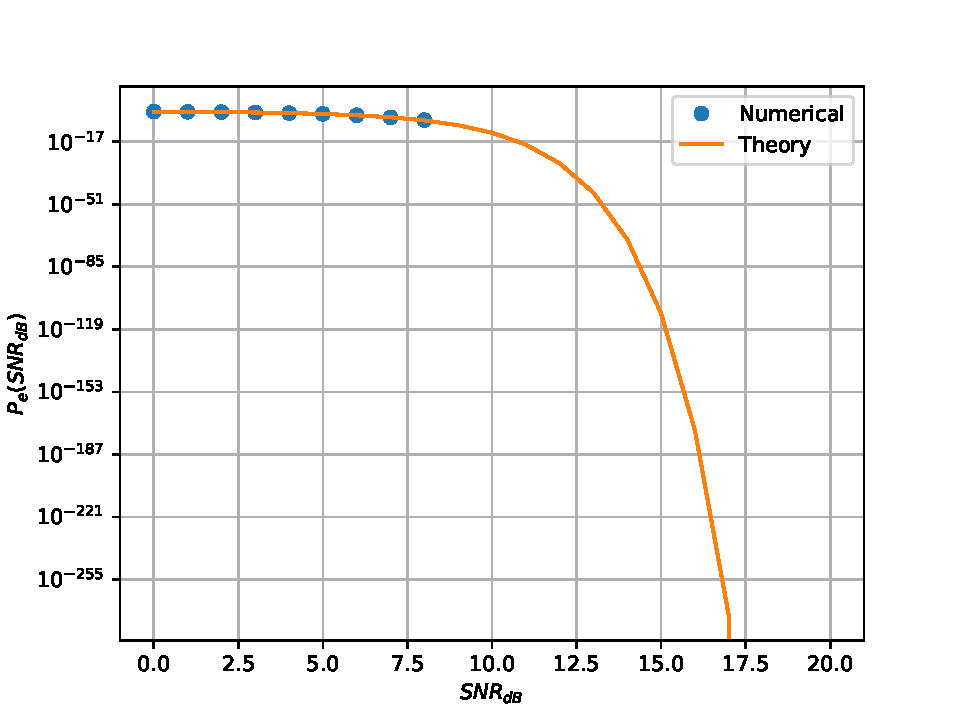
\includegraphics[scale=0.8]{chapter5/figs/biv_pe_vs_snr.pdf}
\caption{$P_e$ with respect to the SNR from 0 to 10 dB}
\label{fig:biv_pe_snr}
\end{figure}
%
\end{enumerate}


\end{document}